\begin{wrapfigure}[0]{r}[9pt]{0cm}
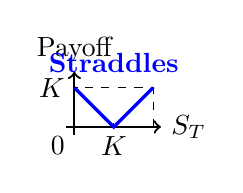
\begin{tikzpicture}[scale=1]
    % --- 定义坐标和参数 ---
    % [修改处] 更新了 K 和 maxST 的范围
    \def\K{0.50}          % 行权价 K
    \def\maxST{1.0}       % S_T 的最大显示范围 (依然是 2K 以展示对称性)
    \def\maxPayoff{\K}    % 在 S_T=0 和 S_T=maxST 时的最大收益

    % --- 绘制坐标轴 ---
    % Y 轴 (Payoff) - 收益始终 >= 0
    % 根据新的 maxPayoff 调整 Y 轴高度
    \draw[->, thick] (0, -0.1) -- (0, \maxPayoff + 0.2) node[above] {Payoff};
    % X 轴 (S_T)
    % 根据新的 maxST 调整 X 轴长度
    \draw[->, thick] (-0.1, 0) -- (\maxST + 0.1, 0) node[right] {$S_T$};

    % --- 绘制辅助线和标签 ---
    % 标记原点
    \node[below left] at (0, 0) {0};

    % 在 X 轴上标记 K
    \draw (\K, 0) node[below] {$K$} -- (\K, 0.05);

    % 在 Y 轴上标记 K (当 S_T=0 时的收益)
    \draw (0, \K) node[left] {$K$} -- (0.05, \K);

    % 绘制辅助虚线以展示对称性
    % 当 S_T = maxST (即 2K) 时，收益也为 K
    \draw[dashed, thin] (\maxST, 0) -- (\maxST, \K) -- (0, \K);


    % --- 绘制 Straddle 收益曲线 (蓝色粗线) ---
    % 路径: (0, K) -> (K, 0) -> (maxST, K)
    % 由于参数是相对的，路径命令不需要修改
    \draw[blue, very thick] (0, \K) -- (\K, 0) -- (\maxST, \K);

    % --- 添加描述标签 ---
    % 标签位置使用相对坐标，会自动跟随 K 调整
    % 左侧腿的描述
    % 右侧腿的描述 (注意这里 maxST 已经是 2K了，所以位置计算需要调整以保持对称)
    % 之前的 1.8*K 在 K=1时是 1.8。现在 K=0.5, maxST=1.0。
    % 我们希望标签在 K 和 maxST 之间。取中点附近: K + 0.8*K = 1.8K.
    % 1.8 * 0.5 = 0.9. 坐标 (0.9, 0.3)

    % --- 添加标题标签 ---
    % 将标题放在图像上方居中位置
    \node[blue, anchor=south, font=\bfseries, yshift=2pt] at (\K, \maxPayoff) {Straddles};

\end{tikzpicture}
\end{wrapfigure}